\documentclass[12pt, a4paper, oneside]{article} 

\usepackage[hyphens]{url}
\usepackage{czech} % nastavení češtiny
\usepackage[center]{caption} 
\usepackage[utf8]{inputenc}
\usepackage{wrapfig} % nastavení obtékání textu
\usepackage{graphicx,amsmath} % nastavení grafiky, matematiky
\usepackage{subfig} % více obrázků vedle sebe 
\usepackage{float}
\usepackage{amsmath}
\usepackage{amssymb}
\usepackage{bbding}
\usepackage{enumitem}
\usepackage{breakurl}
\usepackage{pdflscape}
\usepackage{fancyvrb}
%\usepackage{indentfirst}

\usepackage{tocloft} %přidá tečky do obsahu ke kapitolám /sekcím 
\renewcommand{\cftsecdotsep}{\cftdotsep}

\usepackage[bookmarksopen,colorlinks,plainpages=false,linkcolor=black,urlcolor=blue,citecolor=black,filecolor=black,menucolor=black,unicode=true]{hyperref}

\urlstyle{rm}
%bookmarksopen -- open up bookmark tree 
%colorlinks -- zbarví odkazy (implicitně orámovaný nezbarvený text)
%urlcolor -- barva odkazů (implicitně magenta) 
%linkcolor=black -- barva odkazů v obsahu (implicitně red)


\usepackage{listings}
\usepackage{color}
\usepackage{minted}
\definecolor{lightgray}{RGB}{240,240,240}
\definecolor{darkgray}{rgb}{.4,.4,.4}
\definecolor{purple}{rgb}{0.65, 0.12, 0.82}
\definecolor{darkgreen}{RGB}{0,150,0}

\usemintedstyle{perldoc}
\newminted{js}{linenos=true, bgcolor=lightgray}
\newminted{ini}{linenos=true, fontsize=\footnotesize}

\lstdefinelanguage{JavaScript}{
  keywords={typeof, new, true, false, catch, function, return, null, catch, switch, var, if, in, while, do, else, case, break, for},
  keywordstyle=\color{blue}\bfseries,
  ndkeywords={class, export, boolean, throw, implements, import, this},
  ndkeywordstyle=\color{blue}\bfseries,
  identifierstyle=\color{black},
  sensitive=zr,
  comment=[l]{//},
  morecomment=[s]{/*}{*/},
  commentstyle=\color{darkgreen}\ttfamily,
  stringstyle=\color{red}\ttfamily,
  morestring=[b]',
  morestring=[b]"
}

\lstset{
   backgroundcolor=\color{lightgray},
   extendedchars=true,
   basicstyle=\footnotesize\ttfamily,
   showstringspaces=false,
   showspaces=false,
   numbers=left,
   numberstyle=\footnotesize,
   numbersep=9pt,
   tabsize=2,
   breaklines=true,
   showtabs=false,
   aboveskip=5mm,
   belowskip=7mm,
   captionpos=b
}

\renewcommand{\listingscaption}{Příklad}
\renewcommand{\listoflistingscaption}{Příklady}


% \usepackage{parskip} -- zapne americké odstavce v celé práci

\addtolength{\textwidth}{-2mm} 
\addtolength{\hoffset}{4mm}  % posun textu kvůli kroužkové vazbě  

\setlength{\intextsep}{5mm} % nastavení mezery okolo obrázků

% nastavení příkazu >\figcaption pro popis čehokoli, jako by to byly obrázky 
\makeatletter   
\newcommand\figcaption{\def\@captype{figure}\caption}
\makeatother

\renewcommand\refname{Literatura} 
%\def\bibname{PŘÍLOHA D: Reference}
%\renewcommand\bibname{PŘÍLOHA D: Reference}
% přejmenuje anglický název Reference na české Literatura


%\makeindex % příprava pro výrobu indexu (jestli ho chcete)

%%    VLNKA <fileinput>  KkSsVvZzOoUuAaIi        
% Defaultni  koncovka pro <fileinput> je  ".tex"
%FIXME: haze error
%\cstieon % Vypne chovani vlnky jako tvrde mezery v matematickem rezimu

%%%%%%%%%%%%%%%%%%%%%%%%%%%%%%%%%%%%%%%%%%%%%%%%%%%%%%%%%%%%%%%
%V PROSTŘEDÍ ROVNIC SE NESMÍ VYSKYTOVAT PRÁZDNÝ ŘÁDEK
%
%PROGRAMY VLNKA A CSINDEX SE MUSÍ SPUSTIT SAMOSTATNĚ
%%%%%%%%%%%%%%%%%%%%%%%%%%%%%%%%%%%%%%%%%%%%%%%%%%%%%%%%%%%%%%%

% definice příkazů 
\newcommand{\D}{\medskip \noindent} % nový odstavec v "americkém" formátování 
\newcommand{\B}{\textbf} %tučné písmo
\newcommand{\A}{\mathbf} %tučné písmo v matematickém režimu
\newcommand{\TO}{\ensuremath{\boldsymbol\Omega}} % tučný znak velké omega -- pro ohmy
\newcommand{\I}{\index}  % vytváří položku indexu (asi nepoužijete)
\newcommand{\Deg}[1][]{\ensuremath{{#1}^\circ}} % vysází značku stupně Celsia
\newcommand{\Def}{\footnotesize Definice: \normalsize}
\newcommand{\Pos}{\footnotesize Experiment: \normalsize}
\newcommand{\Odv}{\footnotesize Odvození: \normalsize}
\newcommand{\Vym}{\footnotesize Vymezení pojmu: \normalsize}
\newcommand{\Ob}{obrázek }
\newcommand{\It}{\textit}  % kurzíva
\newcommand{\M}{\mathrm}   % v prostředí rovnic nastaví normální písmo (místo kurzívy ) 
\newcommand{\F}{\footnotesize} % zmenšená velikost písma
\newcommand{\N}{\normalsize} % normální velikost písma
%\newcommand{\U}{\underline}  % podtržené písmo
\newcommand{\e}{\ensuremath} 
\newcommand{\Has}{\textcolor{green}{\CheckmarkBold}}
\newcommand{\NoHas}{\textcolor{red}{\XSolidBrush}}
\newcommand*{\fullref}[1]{\hyperref[{#1}]{\ref*{#1}: \uv{\nameref*{#1}}}}
\DefineShortVerb{\|}
% další příkaz se aplikuje, pouze, když jste v matematickém režimu

%\hyphenation{Pusť-me pla-tí hod-no-ty do-sa-dí-me za-da-né dal-ším}
% dělení slov, kdyby implicitní nevyhovovalo

\linespread{1.3} 
% řádkování 1,5x  
% použijete podle situace  

\unitlength=1mm % nastavení volby jednotek 

% konec hlavičky
%%%%%%%%%%%%%%%%%%%%%%%%%%%%%%%%%%%%%%%%%%%%%%%%%%%%%%%%%%%%%%%%%%%
%%%%%%%%%%%%%%%%%%%%%%%%%%%%%%%%%%%%%%%%%%%%%%%%%%%%%%%%%%%%%%%%%%%

\begin{document} % začátek textové části 

% titulní strana
\pagestyle{empty} % vynechá číslování
 
\voffset = -20mm % posun začátku textu výš
\enlargethispage{60mm} % zvětší oblast tisku pro tuto stránku   

\begin{center}
 
\Large \B{STŘEDOŠKOLSKÁ ODBORNÁ ČINNOST}

\vspace{60mm}

\Huge %\LARGE
\B{MultiROM} \\
\LARGE
\B{Nástroj pro instalaci více operačních systému na mobilní zařízení}
% na titulní straně může být stručnější, pokud je to potřeba  

\Large

\vspace{90mm}


\B{Vojtěch Boček} \\

\vspace{40mm}

\B{Brno 2014}


\end{center}

\newpage % konec titulní strany 
%%%%%%%%%%%%%%%%%%%%%%%%%%%%%%%%%%%%%%%%%%%%%%%%%%%%%%%%%%%%%%%%%%%%%%%%%%%

% vnitřní titulní strana
\voffset = -20mm % posun začátku textu výš
\enlargethispage{60mm} % zvětší oblast tisku pro tuto stránku   

\begin{center}

\Large \B{STŘEDOŠKOLSKÁ ODBORNÁ ČINNOST}  \\
\vspace{10mm}
 \normalsize 
\B{Obor SOČ: 18. Informatika}% číslo a název -- vyplníme spolu 

\vspace{45mm}

\Huge
\B{MultiROM} \\
\LARGE
\B{Nástroj pro instalaci více operačních systému na mobilní zařízení}
\end{center}
\large

\vspace{50mm}


\begin{tabbing}
\hspace{10mm} \= \hspace{30mm}  \=   \kill % nastavení zarážek 
  \> \B{Autor:}  \> \B{Vojtěch Boček}        \\[8mm] 
  \> \B{Škola:}   \> \B{SPŠ a~VOŠ technická, }     \\
  \>              \> \B{Sokolská 1, 602 00 Brno}    \\[8mm]
\end{tabbing}

\vspace{20mm}

\begin{center}
\B{Brno 2014}

\end{center}
\normalsize
%%%%%%%%%%%%%%%%%%%%%%%%%%%%%%%%%%%%%%%%%%%%%%%%%%%%%%%%%%%%%%%%%%%%%%%%%%%
\newpage  % Prohlášení o autorství  
\voffset = 0mm % posun začátku textu zpět

~ % musí to tu být, aby fungovala svislá mezera

\vspace{10mm}

\section*{Prohlášení}

Prohlašuji, že jsem svou práci vypracoval samostatně, použil jsem pouze podklady (literaturu, SW atd.) citované v~práci a~uvedené v~přiloženém seznamu a~postup při zpracování práce je v~souladu se zákonem č. 121/2000 Sb., o~právu autorském, o~právech souvisejících s~právem autorským a~o~změně některých zákonů (autorský zákon) v~platném znění. 
 
\vspace{20mm} 
 
\noindent V~Brně  dne: 6.3.2014 \hspace{50mm}                 podpis:   
 

%%%%%%%%%%%%%%%%%%%%%%%%%%%%%%%%%%%%%%%%%%%%%%%%%%%%%%%%%%%%%%%%%%%%%%%%%%%
\newpage   % Poděkování -- nepovinné 

~ % musí to tu být, aby fungovala svislá mezera
\vspace{100mm}

\section*{Poděkování}
Děkuji Jakubu Streitovi za rady, obětavou pomoc, velkou trpělivost a~podnětné připomínky poskytované během práce na tomto projektu, Martinu Vejnárovi za informace o~programátoru Shupito, panu profesorovi Mgr. Miroslavu Burdovi za velkou pomoc s~prací a~v~neposlední řadě Bc. Martinu Foučkovi za rady a~pomoc při práci s~Qt Frameworkem. Dále děkuji organizaci DDM Junior za poskytnutí podpory.
 

%%%%%%%%%%%%%%%%%%%%%%%%%%%%%%%%%%%%%%%%%%%%%%%%%%%%%%%%%%%%%%%%%%%%%%%%%%%
\newpage   % Anotace 
~ % musí to tu být, aby fungovala svislá mezera
\vspace{-20mm}

\section*{Anotace}

%MultiROM is one-of-a-kind multi-boot mod for Nexus 7. It can boot any Android ROM as well as other systems like Ubuntu Touch, Plasma Active, Bohdi Linux or WebOS port.Besides booting from device's internal memory, MultiROM can boot from USB drive connected to the device via OTG cable. The main part of MultiROM is a boot manager, which appears every time your device starts and lets you choose ROM to boot. You can see how it looks on the left image below and in gallery. ROMs are installed and managed via modified TWRP recovery. You can use standard ZIP files to install secondary Android ROMs, daily prebuilt image files to install Ubuntu Touch and MultiROM even has its own installer system, which can be used to ship other Linux-based systems.

Tato práce popisuje modifikaci pro mobilní zařízení s operačním systémem Google Android, která umožňuje instalaci více operačních systémů vedle sebe, podobně jako na PC. Může to být pouze několik různých verzí OS Google Android, ale i úplně jiné systémy - například právě se vyvíjejicí Ubuntu Touch a další.

Možnost provozovat více operačních systému na jedno zařízení je užitečná spíše pro pokročilé uživatel, podobně jako na stolních počítačích, nicméně počet aktivních uživatelů dokazuje, že zájem o tuto modifikaci rozhodně existuje.

\addtolength{\textheight}{30mm} % prodlouží následující stránku

%%%%%%%%%%%%%%%%%%%%%%%%%%%%%%%%%%%%%%%%%%%%%%%%%%%%%%%%%%%%%%%%%%%%%%%%%%%
\newpage
\pagestyle{plain}

\setlength{\voffset}{-20mm} % posune text/obrázek na této stránce nahoru
\setcounter{page}{1}  % nastaví čítač stránek znovu od jedné

\tableofcontents  % vysází obsah

\addtolength{\textheight}{-30mm} % zkrátí následující stránku
%%%%%%%%%%%%%%%%%%%%%%%%%%%%%%%%%%%%%%%%%%%%%%%%%%%%%%%%%%%%%%%%%%%%%%%%%%%
\newpage
\setlength{\voffset}{0mm} % posune text/obrázek na této stránce, kam patří
%\pagestyle{headings} % znovu zapne číslování
\pagestyle{plain}

%
% Motivace 
\section*{Úvod}
\addcontentsline{toc}{section}{Úvod} % přidá položku úvod do obsahu
\label{uvod}



\section{Motivace}
Abych mohl vysvětlit důvod, proč je multi-boot na mobilních zařízeních užitečný, musím nejdříve upozornit na možnosti, které tato zařízení mají.

Tablety a telefony s platformou Google Android lze narozdíl od jiných systémů relativně snadno upravovat. Uživatelé na nich mohou získat přístup k tzv. superuživateli\footnote{Uživatel, který má práva přistupovat a měnit všechny části systému, je možné ho připodobnit k uživateli \It{Administrátor} v MS Windows. V Linuxu se jmenuje \It{root}.} a dále pak upravovat software na zařízení jakýmkoliv způsobem chtějí. Toto společně s faktem, že velká část OS Android má otevřené zdrojové kódy, vedlo ke vzniku obrovské komunity programátorů a nadšenců, kteří tyto zařízení různými způsoby upravují a vylepšují. Jedním z \uv{produktů} této komunity jsou celé upravené distribuce Androidu, tzv. ROM.

\subsection{Android ROM}
ROM lze přirovnat k distribucím Linuxu, jak je známe ze stolních počítačů. Jejich základem jsou obvykle zdrojové kódy z AOSP\cite{aosp}\footnote{\It{Android Open Source Project} - označení pro otevřenou část zdrojových kódů OS Android}, které si autoři upravují podle svých představ - přidávají optimalizace pro zrychlení celého systému, přidávají další možnosti personalizace pro uživatele, mění prvky uživatelského rozhraní a mnoho dalšího. Na zařízeních, která již nejsou podporované výrobcem, mohou být ROM jediným způsobem, jak na ně přinést novější verze OS Android.

ROM často vydávají a spravují pouze jednotlivci, ale existují i projekty s velkým počtem vývojářů i uživatelů, například CyanogenMod\cite{CM}. Ten nedávno překonal hranici 10 milionů uživatelů, oficiálně podporuje přes 200 zařízení a je aktuálně největší upravenou ROM.

\subsection{Další operační systémy}
Kromě Androidu existují i další mobilní operační systémy, například Ubuntu Touch\cite{utouch}, Mozilla Firefox OS\cite{firefoxos} a další. Tyto systémy často použivají zařízení původně prodávaná s Androidem jako testovací, zejména kvůli jejich snadné dostupnosti a relativně nízké ceně. Pro tablet Google Nexus 7 dokonce existuje plná verze Linuxové distribuce Ubuntu, díky které je možné tento tablet po připojení klávesnice a myši používat jako netbook, s většinou programů které známe z PC.

\begin{figure}[H]
\begin{center}
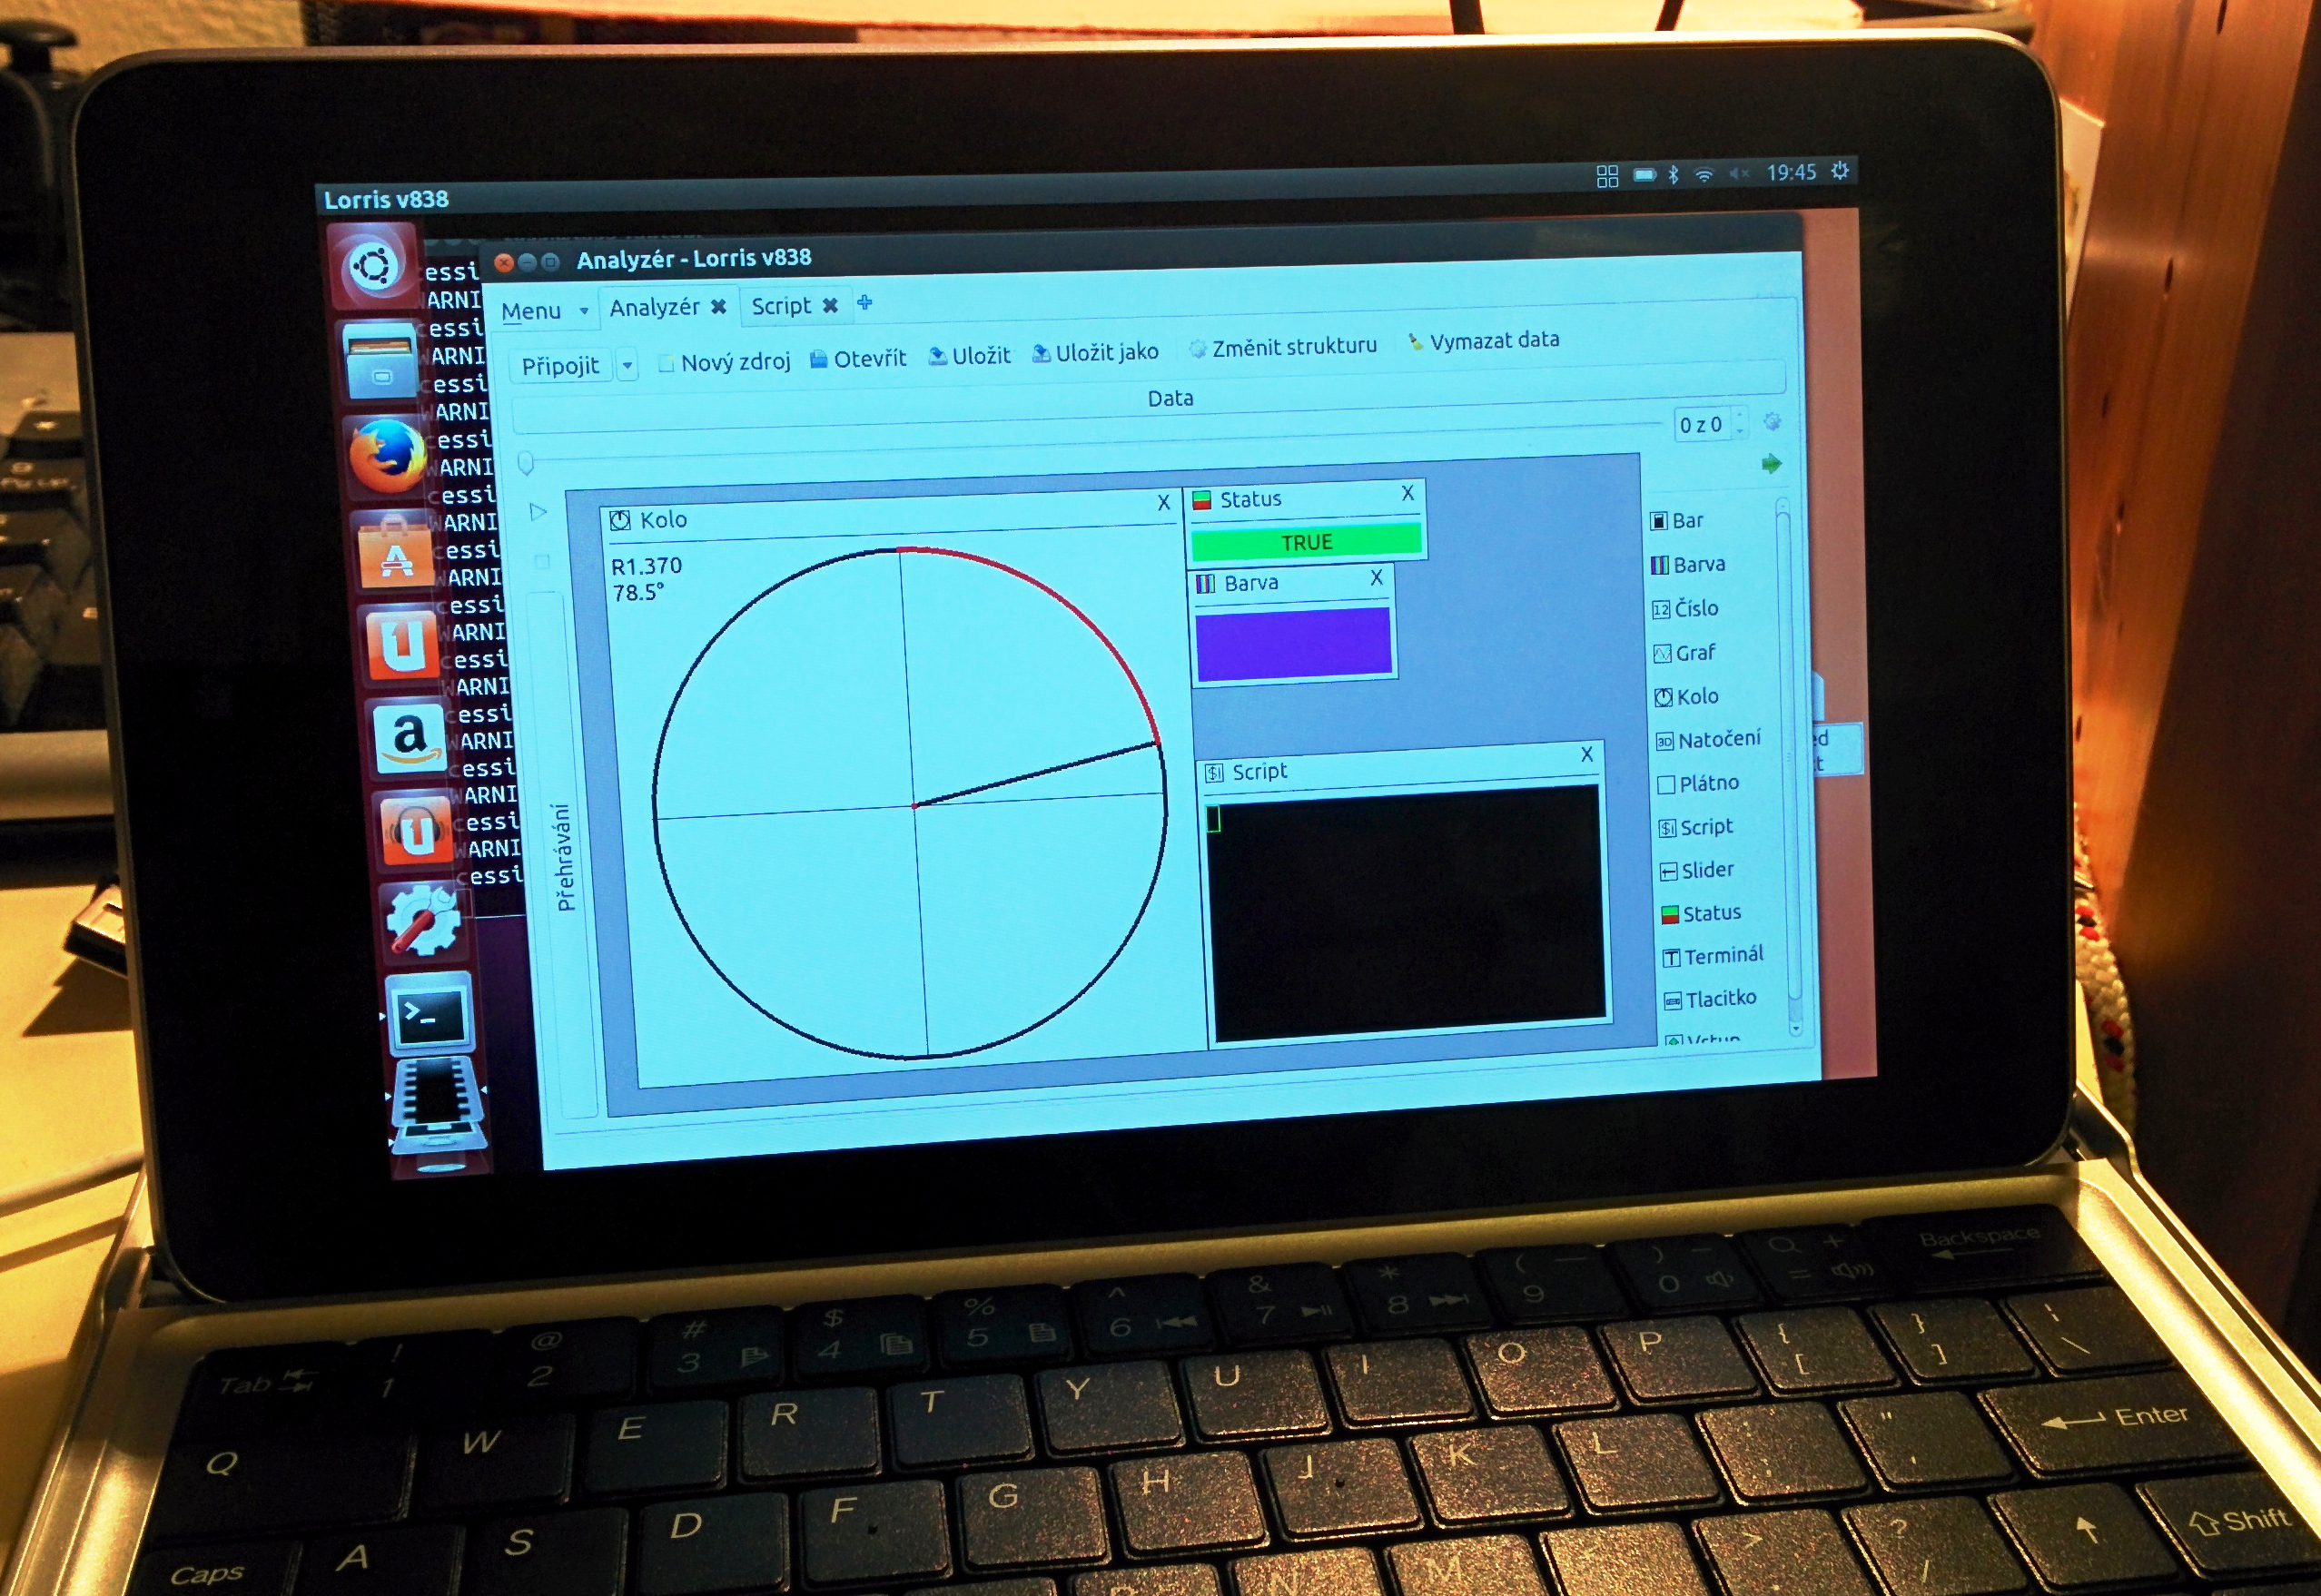
\includegraphics[width=\textwidth]{img/n7_ubuntu.jpg}
\caption{Ubuntu na tabletu Nexus 7 s připojenou klávesnicí}
\end{center}
\end{figure}


\subsection{Více systémů na jednom zařízení}
Tyto telefony a tablety tedy ve většině případů (více o této problematice v příloze \uv{\nameref{sec:locked}}) nejsou uzamknuté na jediném, výrobcem vybraném systému a jeho verzi a dokáží podobně jako stolní počítače provozovat více typů a verzí operačních systémů. Chybí jim však možnost mít více systémů nainstalovaných zárověň (dále jen \It{multiboot}). Tato skutečnost pravděpodobně nevadí běžnému uživateli, nicméně pro zkušené uživatele a vývojáře je \It{multiboot} neocenitelnou funkcí. Mohou ho využít například při:

\begin{itemize}
    \item \B{vývoji aplikací pro Android} - programátoři aplikací pro Android často mají své zařízení odemknuté a systém který používají různými způsoby upravený, nicméně takové prostředí není příliš vhodné pro vývoj aplikací pro většinu uživatelů, která nic takového nepoužívá. S \It{multibootem} mohou mít jeden systém se svými úpravami pro běžné používání a druhý, neupravený, na kterém mohou bez obav testovat své aplikace. \\
    Při psaní aplikací je čas od času třeba vyzkoušet určitou funkcionalitu na jiné verzi OS Android, to je s \It{multibootem} také mnohem jednodušší - není třeba přepsat aktuální systém na zařízení, stačí nainstalovat požadovanou verzi OS jako další operační systém.

    \item \B{zkoušení jiných ROM} - ROM vytvořené komunitou mají v některých případech nové a velmi zajímavé funkce, nicméně je často vhodné vyzkoušet si danou ROM před tím, než uživatel projde zdlouhavým procesem obnovování všech svých dat do této nové ROM. S \It{multibootem} je možné novou ROM jen nainstalovat jako další systém bez toho, aby se smazal ten původní a v případě, že nová ROM uživateli nesedne, může ji kdykoliv smazat. Jeho původní systém se všemi daty je stále neporušený.\\
    Toto platí i pro jiné operační systémy - příkladem budiž Ubuntu Touch od firmy Canonical, nový operační systém s ovládáním značně odlišným od Androidu. Řada uživatelů by si tento OS ráda zkusila, nicméně Ubuntu Touch je stále ve vývoji a není ještě zcela schopný plně nahradit Android. Bez \It{multibootu} by museli museli smazat svůj hlavní OS, což řadu uživatelů odradí.

    \item \B{potřebě využívat aplikace z více operačních systémů} - jako příklad opět použiji Ubuntu Touch, který bych jako nadšenec chtěl používat, nicméně v práci potřebuji určitou aplikaci, která je kompatibilní pouze s OS Android. S \It{multibootem} si nemusím vybírat, stačí přepínat mezi těmito OS podle aktuální situace. Toto použití můžeme pozorovat i na PC, kde má řada uživatelů Linuxu současně nainstalovaný i MS Windows, protože potřebují používat nějakou proprietární aplikaci, která není s Linuxem kompatibilní.
% TODO: doplnit
\end{itemize}

\noindent \It{Multiboot} je tedy užitečný i na přenosných zařízeních, což, jak se přesvědčíte dále v této práci, potvrzuje i počet uživatelů MultiROM.

\section{MultiROM}
MultiROM je modifikace pro zařízení původně s OS Android, která umožňuje používat více operačních systémů zárověň na jednom zařízení. Skládá se ze čtyř částí, které budou dalé důkladně popsány v samostatných kapitolách:

\begin{enumerate}
    \item \B{boot manager} - hlavní část tohoto projektu. Zobrazuje se v průběhu startu zařízení, nechá uživatele vybrat, který operační systém chce spustit a provede akce nutné ke spuštění tohoto systému.
    \item \B{upravená recovery} - tato část se stará o snadnou instalaci a správu nainstalovaných systémů.
    \item \B{kexec-hardboot patch} - modifikace Linuxového jádra, která umožňuje nastartovat jiné jádro z již běžícího, tedy ukončit aktuální operační systém a spustit nový.
    \item \B{aplikace pro Android} - umí rychle a jednoduše nainstalovat všechny potřebné části MultiROM a aktualizovat je a do omezené míry spravovat nainstalované systémy a také do nich přepnout přímo z Androidu (bez nutnosti restartovat zařízení a až poté vybrat systém v boot manageru).
\end{enumerate}

MultiROM je svobodný software, distribuovaný pod licencí GNU GPLv3 (boot manager, recovery a Android aplikace) a GNU GPLv2 (kexec-hardboot patch). Zdrojové kódy jsou k dispozici v repozitářích na serveru GitHub:
\begin{itemize}
    \item \B{Boot manager:} \url{http://github.com/Tasssadar/multirom}
    \item \B{Recovery:} \url{http://github.com/Tasssadar/Team-Win-Recovery-Project}
    \item \B{Android aplikace}: \url{http://github.com/Tasssadar/MultiROMMgr}
\end{itemize}

\subsection{Kompatibilní zařízení}
Platforma ARM bohužel stále není standardizovaná alespoň do takové míry jako x86, kterou známe z PC, a proto není možné vytvořit tuto nízkouúrovňovou modifikaci tak, aby fungovala se všemi Android telefony a tablety. V současnosti oficiálně podporuji tato zařízení:

\begin{enumerate}
    \item Telefon \B{Google Nexus 4}
    \item Telefon \B{Google Nexus 5}
    \item Tablet \B{Google Nexus 7 (verze z roku 2012)}
    \item Tablet \B{Google Nexus 7 (verze z roku 2013)}
\end{enumerate}

Seznam není příliš dlouhý, zejména protože s každým dalším podporovaným zařízením značně narůstá čas, který musím věnovat testování a protože jen velmi nerad podporuji zařízení, které nevlastním - jak jsem se přesvědčil u Nexusu 4, značně to omezuje schopnost řádně otestovat nové funkce a úpravy, protože musím spoléhat na některého ze zkušenějších uživatelů MultiROM, aby vše řádně otestoval, případně pomohl s řešením problému.

MultiROM má ale svobodný zdrojový kód, takže kdokoliv může přidat podporu pro další zařízení, což se také stalo - existují neoficiální verze například pro telefony HTC One, Samsung Galaxy S3 nebo Sony Xperia M. Verze pro Nexus 4 byla původně také upravena jiným členem komunity, já jsem ji převzal a poskytuji pro ni podporu.

\subsection{Požadavky}
MultiROM mění části systému, zařízení tedy musí být odemknuté. Všechny oficálně podporované přístroje patří do řady Nexus, jsou tedy \uv{volně odemykatelné} (více o této problematice v příloze \uv{\nameref{sec:locked}}).

MultiROM aplikace pro Android vyžaduje, aby bežela na systému s přístupem k \It{superuživateli}, protože potřebuje přistupovat do částí systému, které nejsou běžným aplikacím přístupné.

Naprostá většina potenciálních uživatelů MultiROM již tyto požadavky splňuje, situace kdy uživatel odemyká své zařízení jen kvůli MultiROM není příliš častá.

\newpage
\section{Boot manager}
Hlavní část MultiROM, která se spustí okamžitě po startu Linuxového jádra, na kterém Android běží, ještě před tím než se začne spouštět samotný Android. Uživatel v ní může vybrat, který systém chce použít a boot manager poté provede akce potřebné ke spuštění vybraného systému.

\begin{figure}[H]
\begin{center}
 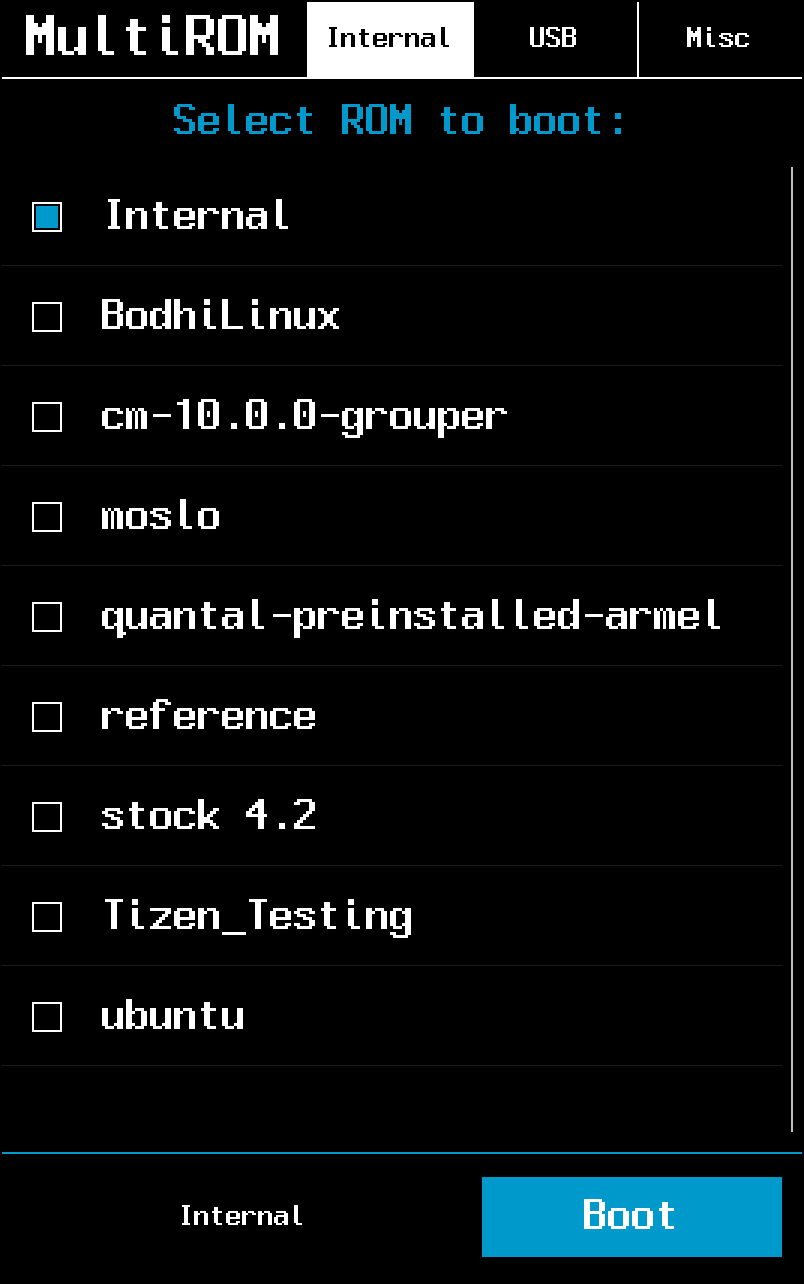
\includegraphics[width=250px]{img/boot_manager.png}
\caption{Obrazovka boot manageru s výběrem systému}
\end{center}
\end{figure}


\section{Upravená recovery}
\subsection{Obecné představení pojmu}
Pojem \uv{recovery} u zařízení s OS Android označuje velmi malý (v řádech několika megabajtů), oddělený systém, původně určený pro instalaci aktualizací OS od výrobce, případně reinstalaci systému v případě jeho porušení. Recovery je obvykle možné spustit vypnutím zařízení a následným podržením určité kombinace tlačítek (např. vypínací tlačítko a tlačítko pro zvýšení hlasitosti zároveň). S podobným nápadem se můžeme setkat i u PC, kdy je na \uv{Oddílu pro obnovu} kopie operačního systému, ze které lze obnovit ten hlavní.

Komunita možnosti recovery značně rozšířila a vylepšila a v současné době existuje několik konkurenčních upravených recovery. Právě přes upravené recovery se instalují ROM vydané členy komunity, umí zálohovat celé zařízení a mají řadu dalších funkcí.

\subsection{TeamWin Recovery Project}
% TODO: screenshot
TeamWin Recovery Project\cite{twrp} (dále jen TWRP) je jedna z upravených recovery a pravděpodobně má nejvíce funkcí. Má grafické rozhraní plně podporující dotykový displej, podporuje témata (celé GUI je napsané pomocí XML souborů a je možné ho jakkoliv upravit), dokáže instalovat ROM, dělat zálohy, mazat diskové oddíly, obsahuje jednoduchý terminál a další.

% TODO: doplnit

\subsection{Jak MultiROM využívá TWRP}
TWRP je svobodným softwarem a kdokoliv do ní může přispívat a používat její zdrojové kódy, což mi umožnilo použít ji ke správě systémů nainstalovaných v MultiROM. TWRP jsem za tímto účelem značně upravil a při práci na ní jsem vytvořil i několiv oprav a úprav, které bylo možné zaslat i do hlavního vývojového stromu TWRP.

Pomocí upravené TWRP se tedy instalují a spravují vedlejší systémy a upravuje se v ní nastavení MultiROM. Za tímto účelem jsem vytvořil v TWRP další položku menu, pod kterou jsou všechny tyto funkce k dispozici, rozhraní již existujících částí recovery je změněné jen minimálně, takže návyky uživatelů z původní TWRP stále platí.

Grafické rozhraní TWRP mi umožnilo vytvořit relativně snadný a rychlý způsob instalace vedlejších ROM - stačí zvolit typ systému, umístění instalace (kromě interní paměti dokáže MultiROM bootovat i z USB flash disku) a instalační soubory, o zbytek se postará recovery.

\subsection {Podporované formáty instalačních souborů}
\B{Android ROM} se instalují pomocí ZIP souborů obsahujících systém a script, který recovery spustí. Tento způsob, pojmenovaný \It{Edify script}, původně používal Google pro instalaci aktualizací přes recovery, nicméně komunita ho velmi rychle adoptovala a používá se k instalaci naprosté většiny Android ROM.

\B{Ubuntu Touch} má dva způsoby instalace - první, starší, používá dva ZIP soubory s \It{Edify scriptem}, moje upravená TWRP umožňuje uživateli vybrat oba soubory na začátku instalace (nemusí je instalovat postupně) a provede během instalace všechny změny potřebné pro běh s MultiROM. Druhý způsob je nový a používá oddělené datové soubory a soubor s příkazy, který zpracovává script v recovery - tento způsob instalace je třeba provádět přes aplikaci pro Android, protože pro stažení instalačních souborů je třeba parsovat určitá metadata (který datový soubor patří ke které verzi systému, ...).

\B{Ubuntu Desktop} pro Nexus 7 (2012) je distribuován jako obraz diskového oddílu. Moje upravená TWRP ho dokáže rozbalit, nainstalovat a upravit tak, aby běžel v prostředí MultiROM. 

\B{MultiROM Instalátor} - nový typ instalačních souborů, který jsem vytvořil speciálně pro MultiROM. Jedná se o nekomprimovaný ZIP archiv, který obsahuje datové soubory (archivy .tar.gz), soubor s informacemi pro MultiROM (podporované souborové systémy, příkazová řádka jádra, ...) a může obsahovat i scripty v jazyce bash, které mohou být spuštěny v různých bodech instalace a udělat, co je pro daný systém potřeba. Více o instalátoru najdete v příloze \uv{\nameref{sec:installer}}.

\section {Kexec-hardboot patch}
\subsection{Kexec}
Kexec je funkce Linuxového jádra, která umožňuje spustit jiné jádro bez nutnosti restartu počítače. Staré jádro se ukončí a místo něj se spustí nové, vynechá se tak fáze startu BIOSu a zavadeče. Restart zařízení pomocí volání kexec je tedy rychlejší, nicméně MultiROM kexec využívá z jiného důvodu.

MultiROM při spouštění jiného systému potřebuje nahrát jeho jádro, ideálně bez toho, aby přepsala jádro hlavního OS, které je uložené v zaváděcím sektoru. Právě k tomu je využit kexec - nové jádro je pouze načteno do operační paměti a spuštěno.

\subsection{Kexec-hardboot}
Kexec potřebuje, aby všechny ovladače při ukončení jádra zanechaly zařízení ve správném stavu tak, aby je nové jádro mohlo znovu inicializovat a použít. Bohužel, ovladače na zařízení s Androidem často nejsou na kexec připraveny a přístroj při pokusu tuto funkci použít jednoduše zamrzne někde mezi starým a novým jádrem. V tomto stavu není možné bez speciálního vybavení a dokumentace nijak zjistit příčinu zamrznutí, opravení ovladačů je tedy téměř nemožné.

Proto byla vytvořena modifikace funkce kexec, nazvaná kexec-hardboot, která přidává do procesu reálný restart zařízení. Staré jádro tedy uloží nové do oblasti operační paměti, která se při restartu nepřepíše a restartuje zařízení. Zavaděč poté korektně nastaví všechny zařízení do počátečního stavu (jako při normálním bootu), několik prvních instrukcí jádra ze zaváděcího sektoru detekuje, že bylo do operační paměti uloženo jiné jádro a přeskočí do něj.

Tento patch původně napsal Mike Kasick\cite{kexec-hardboot-orig}, já jsem ho upravil pro zařízení podporované MultiROM a také významně vylepšil jeho možnosti (podrobně popsáno v příloze  \uv{\nameref{sec:kexec-hardboot}})

\section{Aplikace pro Android}
Aplikace \It{MultiROM Manager} je poměrně nová část MultiROM, přidaná hlavně za účelem zjednodušení instalace celé modifikace. Postupně přibyla instalace Ubuntu Touch, možnost správa instalovaných systémů a možnost nabootovat do systému přímo z této aplikace, bez nutnosti restartovat nejdříve do boot manageru.

\subsection{Instalace a aktualizace MultiROM}
Aplikace dokáže vše potřebné (MultiROM, Recovery a kernel) stáhnout a nainstalovat. Dále hlídá, jestli jsou verze všech komponent aktuální a v případě že nejsou, nabídne uživateli aktualizaci. Kvůli této funkci jsem vytvořil server, který hostuje data o dostupných verzích pro jednotlivé zařízení a skladuje všechny instalační soubory.

Tato část aplikace výrazně zjednodušila instalaci a aktualizace celého projektu - dříve byly aktualizace vydávány pouze na XDA fóru a uživatel na si muesel aktualizace všimnout, stáhnout ji, nahrát do telefonu a nainstalovat. MultiROM Manager tohle všechno zvládá v jednom kroku.

\begin{figure}[H]
\begin{center}
 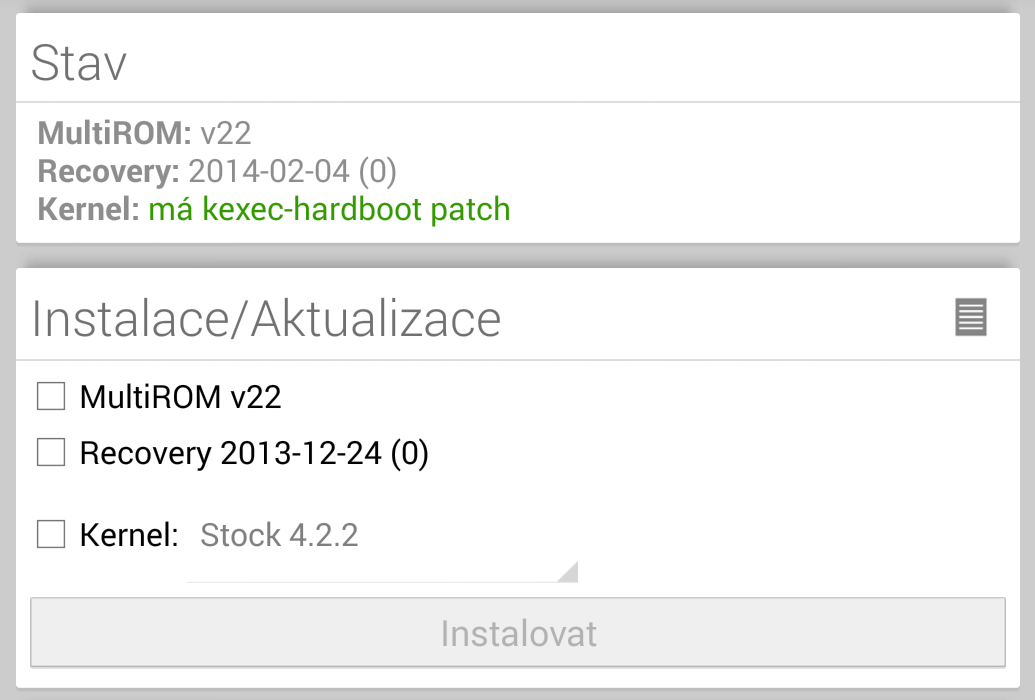
\includegraphics[width=\textwidth]{img/mgr_install.png}
\caption{Instalace a aktualizace v manageru}
\end{center}
\end{figure}

\subsection{Instalace Ubuntu Touch}
Původně Ubuntu Touch používalo ke své instalaci ZIP soubory s \It{Edify} scriptem, podobně jako Android ROM. Jeho vývojáři ale přešli na nový systém, skládájící se z obrovské složky s nečitelně pojmenovanými datovými soubory a z metadat, které určujů, který datový soubor patří ke které verzi OS a ke kterému zařízení. Uživatel samotný bez jakéhokoliv nástroje se mezi datovými soubory nemůže vyznat a stáhnout ten správný, a tak Ubuntu používá na instalaci na nařízení scripty. Ty beží na počítači, naparsují metadata, stáhnou příslušné datové soubory a nainstalují je na zařízení připojené k počítači přes USB. Tyto scripty samozřejmě nejsou kompatibilní s MultiROM, a proto jsem do MultiROM Manageru přidal funkci instalace Ubuntu Touch jako další vedlejší systém.

Manager naparsuje metadata, stáhne všechny potřebné soubory podle vybrané verze a nainstaluje je jako další systém do MultiROM.

\begin{figure}[H]
\begin{center}
 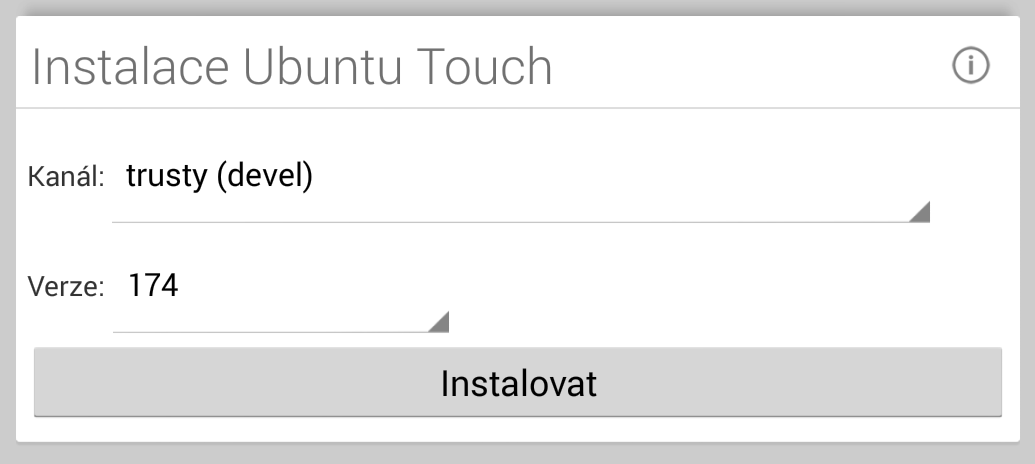
\includegraphics[width=\textwidth]{img/mgr_ubuntu.png}
\caption{Volby instalace Ubuntu Touch}
\end{center}
\end{figure}


\section {Princip multibootu}
\label{princip-multibootu}
MultiROM instaluje všechny vedlejší operační systémy do podsložky na \uv{kartě SD}\footnote{Řada zařízení již fyzickou SD kartou nedisponuje, \uv{SD kartou} se tedy označuje část vnitřní paměti přístroje, která kartu nahrazuje}. Každý systém má svoji vlastní podsložku, která je později funguje jako kořen tohoto systému místo původního, hlavního kořene. Další postup se liší podle typu systému.

\subsection{Android}
OS Android má proces startu systému a uspořádání systému souborů odlišné od běžných Linuxových distribucí. Jádro systému si ihned po startu rozbalí archiv souborů do operační paměti a použije ho jako kořen souborového systému. Tento archiv je běžně označován jako \It{init ramdisk}, zkráceně \It{initrd}. \It{Initrd} obsahuje první program, který se spustí po startu jádra systému, tvz. \It{init}. Tento má za úkol inicializovat zařízení v telefonu, připojit všechny \uv{diskové oddíly} a spustit z nich zbytek Androidu, k čemuž používá \It{scripty}, které čte a vykonává akce v nich definované.

Před ním než budu pokračovat, musím upozornit na to, že Android používá tři hlavní diskové oddíly: \B{/data}, pro aplikace a uživatelská data, \B{/system}, pro nainstalované neměnné části systému a \B{/cache} pro dočasné soubory. Nahrazení všech těchto složek jinými prakticky znamená spuštění jiného systému.

MultiROM \B{nahrazuje} \It{init} v \It{initrd}, je tedy prvním programem, který běží po startu jádra. Poté, co uživatel vybere systém, který chce spustit, boot manager provede následující proces:
%buďto použije kexec k restartování zařízení s jádrem vybraného systému nebo pokračuje dále s již spuštěným jádrem, které se tedy sdílí mezi hlavní a vedlejší ROM (možné nastavit při instalaci ROM). 

\begin{enumerate}
    \item Použije kexec k:
    \begin{enumerate}
        \item \B{restartování zařízení s jádrem vybraného systému} nebo
        \item \B{pokračuje dále se stejným jádrem}, které se tedy sdílí mezi hlavní a vedlejší ROM (možné nastavit při instalaci ROM).
    \end{enumerate}
    \item Přípojí podsložky vybrané ROM z SD karty na umístění v kořenu souborového systému, tedy /data, /system a /cache.
    \item Přepíše scripty původní ROM těmi z uživatelem vybrané ROM.
    \item \B{Upraví scripty tak, aby již nepřipojovali původní diskové oddíly na /data, /system a /cache} - přepsali by složky vedlejší ROM, které boot manager již připojil.
    \item Boot manager se ukončí a \B{spustí místo sebe \It{init} z uživatelem vybrané ROM}, který spustí tuto ROM ze složek, které boot manager připojil na /data, /system a /cache.
\end{enumerate}
%TODO obrázek

Multiboot systému Android je poměrně přímočarý a MultiROM ho zvládne provést sama, není třeba danou ROM nijak modifikovat aby byla s MultiROM kompatibilní.

\subsection{Ostatní systémy}
MultiROM zvládne nabootovat jakýkoliv systém založený na Linuxovém zařízení (žádný jiný druh není pro tato zařízení k dispozici), ale je potřeba tyto systémy modifikovat, aby dokázali použít podsložku SD karty jako kořen systému souborů. Boot manager spouští tento typ systémů následujícím způsobem:
\begin{enumerate}
    \item Použije kexec k \B{restartování zařízení s jádrem a \It{initrd} vybraného systému}. Nastaví přitom do příkazové řádky jádra\footnote{Několik textových parametrů jádra, např. "\verb-console=tty1 root=/dev/sda1 rootfstype=ext4 debug-"} \B{cestu do složky s kořenem spouštěného systému}
    \item Po restartu již MultiROM systém \B{nijak neovlivňuje}. Je na systému samotném, aby jako kořenový systém připojil složku, která mu byla předána v příkazové řádce jádra.
\end{enumerate}

MultiROM hledá jádro systému a \It{initrd} a předává jádru parametry podle informací v souboru |rom_info.txt|, umístěného v adresáři tohoto vedlejšího systému. Jak |rom_info.txt| vypadá můžete vidět v příkladu \ref{rom-info}.

Tento typ systémů tedy musí byt upraven tak, aby byl schopný připojit složku předanou v příkazové řádce jádra jako kořen souborového systému. Jedná se obvykle o poměrně nenáročnou úpravu jednoho ze scriptů programu \It{init}, které většina OS založených na Linuxu má (ale nejsou všechny stejné, proto není možné upravovat je z MultiROM). V případě Ubuntu Touch dokáže recovery při instalaci systém patřičně upravit, je tedy možné použít původní, neupravené instalační soubory.

\linespread{1.1}
\begin{listing}[H]
\begin{inicode}
# So far, the only supported ROM type for these files is kexec-based linux
type="kexec"

# Paths to root of the ROM.
# Both image and folder can be specified at one time, MultiROM will use 
# the one which it can find. If both are present, folder is used.
# Must _not_ contain spaces.
# Path is from root of the root partition, but you will usually want
# to use following alias:
# - %m - ROM's folder (eg. /media/multirom/roms/*rom_name*)
root_dir="%m"
root_img="%m/data.img"
root_img_fs="ext4"

# Path to kernel and initrd. Kernel path _must_ be specified.
# Paths are relative to the folder in which is this file
# Those can be outside the root folder/image, or use %r if it is in there:
# kernel_path="%r/boot/vmlinuz"
# If ROM is in images, it will mount the image and load it from there.
# You can use  * _at the end of the filename_ as wildcard character.
kernel_path="zImage"
initrd_path="initrd.img"

# Set up the cmdline
# img_cmdline and dir_cmdline are appended to base_cmdline.
# Several aliases are used:
#  - %b - base command line from bootloader. You want this as first
#         thing in cmdline.
#  - %d - root device. is either "UUID=..." (USB drive) or
#         "/dev/mmcblk0p9" or "/dev/mmcblk0p10"
#  - %r - root fs type
#  - %s - root directory, from root of the root device
#  - %i - root image, from root of the root device
#  - %f - fs of the root image
base_cmdline="%b console=tty0 androidboot.hardware=hammerhead ..."
img_cmdline="loop=%s loopfstype=%f"
dir_cmdline="rootsubdir=%s"
\end{inicode}
\caption{Obsah souboru \textt{rom\_info.txt} s komentáři}
\label{rom-info}
\end{listing}

\linespread{1.3}

\section{Srovnání s jinými multiboot nástroji}
Žádný jiný multiboot nástroj pro zařízení řady Nexus, které MultiROM podporuje, neexistují, budu tedy srovnávat s metodamy, které jsou běžné pro jiné telefony a tablety.

Nejčastějším způsobem je tzv. \B{dual-boot kernel}, který spočívá upravení \It{init} skriptů a používání některé z volných oddílů na zařízení pro umístění druhé ROM (například |/cache|). Do druhého systému se uživatel nabootuje, pokud bude držet některou z kláves na zařízení, např. snížení hlasitosti. Nevýhody této metody jsou možnost instalace pouze dvou systémů, které navíc musí být jen Android ROM. Dále používá pro obě ROM stejné jádro, které tedy musí být s oběma kompatibilní.

Méně častá jsou \B{řešení založená na volání kexec}, podobně jako MultiROM. Pro ukládání vedlejších ROM používají obrazy oddílů nebo složky a často mají i nějakou formu boot manageru. Jako příklad použiji modifikaci \It{Xperia Boot Menu}\cite{xperia-boot-menu}, která používá kexec-hardboot patch, nicméně nemá upravenou recovery, který by pomáhala s instalací vedlejších ROM, která se tím pádem stává poměrně náročnou činností.

Dalším populární modifikací je MoDaCo.SWITCH\cite{modaco-switch}, jejíž hlavní předností je sdílení všech dat a aplikací mezi hlavním a vedlejším systémem. Jedná se však pouze o dual-boot, a to jen mezi dvěma ROM - uživatel si je nemůže vybrat, protože jsou součástí této modifikace. Právě to umožňuje relativně bezproblémové sdílení všech dat mezi oběma systémy, které MultiROM ještě nepodporuje.

Mezi hlavní výhody MultiROM patří zejména \B{velmi snadná instalace a používání} v porovnání s ostatními podobnými modifikacemi. Aplikace pro Android nainstaluje vše potřebné a udržuje MultiROM aktualizovanou a další systémy se instalují v upravené recovery velmi podobně jako bez multibootu - stačí pouze vybrat ZIP soubor a stisknout tlačítko. MultiROM dále podporuje téměř \B{jakýkoliv typ operačního systému} - například pro Nexus 7 existují kromě Androidu balíčky se systémy Ubuntu Touch, Ubuntu Desktop, Plasma Active, WebOS, Tizen, BohdiLinux či ArchLinux. Další důležitou vlastností je možnost \B{instalace jakéhokoliv množství vedlejších systémů}, jediným limitem je velikost paměti. Navíc je možné \B{instalovat i na USB flash disk}, pokud je interní paměť zařízení vyčerpána.

\section{Přijetí MultiROM}
\subsection{XDA Developers fóra}
Server \url{http://xda-developers.com} je největším webem zabývajícím se upravováním Android (ale i jiných) zařízení. Jeho hlavní částí je fórum, kde vývojáři a nadšenci vydávají své produkty. Právě zde lze nalézt nejvíce různých druhů ROM a dalších modifikací.

Hlavním způsobem, jak získává MultiROM nové uživatele a já komunikuji s existujícími jsou právě vlákna na XDA fóru. Obsahují popis MultiROM, návod na instalaci, návod k používání, seznam změn a odkazy ke stažení. Každé zařízení má svě vlastní vlákno:

\begin{itemize}
\item Nexus 7 (2012):\\ \url{http://forum.xda-developers.com/showthread.php?t=2011403}
\item Nexus 7 (2013):\\ \url{http://forum.xda-developers.com/showthread.php?t=2457063}
\item Nexus 4: \url{http://forum.xda-developers.com/showthread.php?p=46223377}
\item Nexus 5: \url{http://forum.xda-developers.com/showthread.php?t=2571011}
\end{itemize}

\subsection{Indiegogo kampaň}
Server indiegogo.com\cite{indiegogo} se zaměřuje na tzv. crowdfunding - jednotlivec či skupina si může na tomto serveru založit projekt, který chtějí vytvořit a stanoví částku kterou potřebují k jeho realizaci. Návšťevníci indiegogo přispívají peníze projektům, které se jim líbí. Záleží pouze na nich kolik přispějí - \$5, \$20 nebo \$10000, jakákoliv částka je možná. Pokud přispěje dostek lidí, mohou uspět i velmi finančně náročné projekty (v řádech milionů dolarů). Důležité je však uvědomit si, že se nejedná o obchod - i když projekt dostane požadovanou částku peněz, není jisté že uspěje, zejména protože crowdfunding dává příležitost podnikat i lidem, kteří nemají žádné zkušenosti. Pokud ale jde vše podle plánu, vznikají často zajímavé projekty, které by jinak umřely jen protože se nelíbily investorům. Projektem může být takřka cokoliv, například počítačová hra, nějaký nový kus hardwaru, ale i vydání prvního alba amatérské kapely či peněžní sbírky pro příspěvkové organizace.

Po vydání nové verze tabletu Nexus 7 v roce 2013 jsem zaznamenal poměrně velké množství požadavků aby MultiROM podporovala i toto zařízení. Poskytnout takovou úroveň podpory (zejména řešení problémů pokud něco nefunguje) je však takřka nemožné, pokud zařízení nevlastním a nemohu na něm vše testovat. Založil jsem tedy na indiegogo projekt na zakoupení Nexusu 7 a přidaní kompatibility pro toto zařízení\cite{indiegogo-multirom}. Cílem byla částka \$500 (menší indiegogo nepodporuje). \B{Kampaň byla úspěšná}, celkově se vybralo \$562 dolarů a \B{já jsem svůj \uv{závazek} splnil, a to i v odhadovaném čase} - verze pro Nexus 7 byla vydána necelý měsíc po skončení kampaně.

% FIXME: zmenšit?
\begin{figure}[H]
\begin{center}
 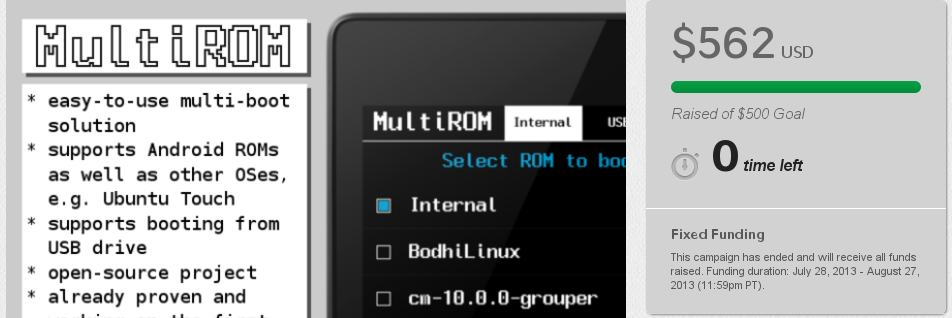
\includegraphics[width=\textwidth]{img/indiegogo.png}
\caption{Výsledek kampaňe na Indiegogo.com}
\end{center}
\end{figure}

\subsection{Počet uživatelů}
Ke každé aplikaci v Obchodě Google Play jsou dostupné i poměrně podrobné statistiky aktivních uživatelů, a tak od vydání aplikace pro Android mohu sledovat i počet uživatelů MultiROM. Tyto statistiky nejsou úplně přesné, protože nezahrnují uživatele, kteří nemají aplikaci nainstalovanou (aplikace není nutnou součástí MultiROM, pouze usnadňuje její používání) ani uživatele některého z mnou nepodporovaných zařízení.

Na grafu č. \ref{graf-uzivatele} můžete vidět graf \B{aktivních} instalací (nezarhnuje tedy zařízení, ze kterých byla aplikace odinstalována) ke dni 2.\,3.\,2014. Poslední hodnota je 12 296 instalací. Dále graf č. \ref{graf-devices} znázorňuje počet instalací podle typu zařízení.

\begin{figure}[H]
\begin{center}
 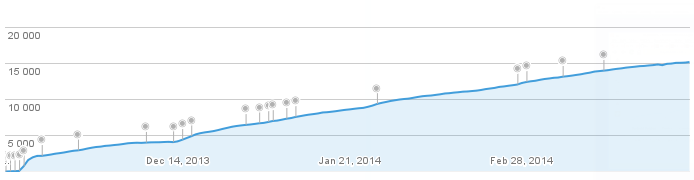
\includegraphics[width=\textwidth]{img/graph_active.png}
\caption{Graf znázorňující nárůst aktivních instalací}
\label{graf-uzivatele}
\end{center}
\end{figure}

\begin{figure}[H]
\begin{center}
 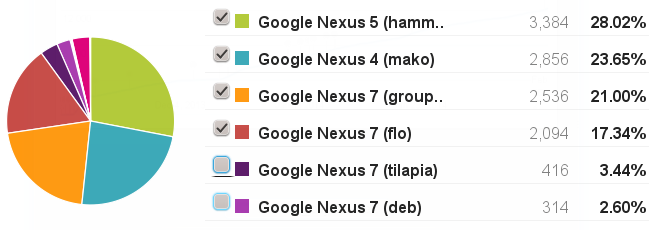
\includegraphics[width=\textwidth]{img/graph_devices.png}
\caption{Graf s počtem instalací podle zařízení}
\label{graf-devices}
\end{center}
\end{figure}

\subsection{Napsali o MultiROM}
\noindent \uv{...A great thing about MultiROM is the way it doesn’t require a lot of tweaking on the user’s part to get things to work...}

\hfill \It{AddictiveTips\cite{addictivetips}} \\

\noindent \uv{...The Nexus 7 by itself is a great ... tablet. However, ... there's a lot of alternate OSes out there for it. MultiROM lets you try them all without requiring you to wipe your device each time you want to try a new OS or ROM build.}

\hfill \It{Linux Journal\cite{linuxjournal}} \\

\noindent \uv{...The Nexus 7 is one of the best devices for a few reasons ... So, how could you make something this good even better? XDA Recognized Developer Tasssadar can answer this question with his latest creation: Multi-Boot for the Nexus 7.}

\hfill \It{XDA-Developers portal\cite{xda-multirom}} \\

\noindent \uv{Do you love to try out different ROMs on your Nexus 7? ... it can get a bit frustrating flashing backwards and forwards between new ROMs and your daily driver. There is an easier way! MultiROM allows you to have multiple ROMs installed on your device and gives you the ability to switch between them at will.}

\hfill \It{AndroidMagazine\cite{androidmagazine}} \\

\noindent \uv{Žonglér s ROM - S MultiROM můžete na váš Nexus 7 nainstalovat několik systémů zároveň, a to jak Android ROM tak další Linuxové distribuce.} (Překlad z němčiny.)

\hfill \It{číslo 21/2013 německého tištěného časopisu c't magazin\cite{ctmagazine}} \\

\noindent \uv{MultiROM is extremely easy to use, even for users with little knowledge, and that is why that stands out other similar tools that require fiddling a bit more about the system by yourself.}

\hfill \It{Firefox OS Guide\cite{firefoxosguide}} \\

\noindent \uv{...But you don’t have to wipe the stock Android software that comes with the tablet to load Ubuntu, CyanogenMod, or another OS. Instead, you can use a new tool called MultiROM to load more than one OS on the 7 inch tablet...}

\hfill \It{Liliputing\cite{liliputing}} \\

\noindent \uv{It’s great to see this extremely useful tool evolving and even better to see the development team recognizing the needs of their users and improving the experience as well as adding additional power.}

\hfill \It{Renmond pie\cite{redmondpie}} \\

\noindent \uv{MultiROM: Must-Have for Nexus 7 Tinkering}

\hfill \It{AppsLab\cite{appslab}}

\newpage
\section*{Závěr}
\addcontentsline{toc}{section}{Závěr}



%%%%%%%%%%%%%%%%%%%%%%%%%%%%%%%%%%%%%%%%%%%%%%%%%%%%%%%%%%%%%%%%%%%%%%%%%%%
\newpage
\section*{PŘÍLOHA A:}
\section*{Uzamykání zařízení pouze na určitý systém}
\addcontentsline{toc}{section}{PŘÍLOHA A: Uzamykání zařízení pouze na určitý systém}
\label{sec:locked}
I když zdrojové kódy OS Android jsou z velké části otevřené, mezi výrobci panuje trend uzamykaní zařízení tak, aby mohli uživatelé používat pouze systém vydaný výrobcem, ať už v zájmu bezpečnosti, zachování určitých vlastností systému (např. předinstalované aplikace často obtěžující uživatele) nebo z prostého nepochopení trhu. V současnosti existuje několik typů uzamknutí zařízení:

\begin{enumerate}
    \item \B{Volně odemykatelné} - uživatel si je může sám odemknout, bez žádných nevýhod oproti uzamknutým zařízením. Tento typ je nejvíce ojedinělý, příkladem jsou zařízení z řady \It{Nexus} vydávané pod záštitou firmy Google.
    
    \item \B{Odemykatelné za registraci} - výrobce provozuje web, který po zadání sériového čísla zařízení vydá odemykací kód. Takto si vytvoří databázi odemknutých zařízení, kterou poté může využít k zamítnutí reklamací (podobné chování nemusí být v souladu s legislativou).
    
    Někteří výrobci při tomto odemknutí smažou klíče pro placený obsah (tzv. DRM\footnote{\It{Digital Rights Management} - systémy navrhnuté pro zabránění nelegálního kopírování digitálního obsahu - hudby, filmů, her apod.}), protože je na odemknutých systémech podle jejich názoru větší nebezpečí nelegálního kopírování obsahu chráněného pomocí DRM.
    
    \item \B{\uv{Edice pro vývojáře}} - výrobce kromě standardní varianty zařízení vydávají verzi, kterou je možné odemknout, buďto za registraci nebo volně. Tyto edice jsou často bezdůvodně dražší anebo nejsou dostupné ve všech zemích, ve kterých je možné koupit standardní variantu. Označení \uv{Developer edition}, které výrobci používají, je v tomto případě mírně zavádějící - zařízení je možné pouze odemknout a kromě této skutečnosti není o nic více přispůsobené vývojářům (části s uzavřeným zdrojovým kódem jsou stále nedostupné a hardware telefonu je rovněž stejný).

    \item \B{Bez možnosti odemknutí} - výrobce neposkytuje žádný způsob jak zařízení odemknout. V naprosté většině případů ale komunita překoná toto omezení a existuje více nebo méně pohodlná možnost neoficiálního odemknutí. Někteří výrobci tomuto odporují a dokonce přidávají vlastnosti kontrolující integritu systému a sledující, zda nebylo uzamknutí prolomeno. Tyto ochrany bývají často také překonány.
    
\end{enumerate}

\newpage
\section*{PŘÍLOHA B:}
\section*{MultiROM instalátor}
\addcontentsline{toc}{section}{PŘÍLOHA B: MultiROM instalátor}
\label{sec:installer}
MultiROM instalátor je formát instalačních souborů, který jsem vyvinul pro MultiROM. Android ke obvykle instalovaný ze ZIP souborů s edify scriptem, je tedy zaměřený zejména na ostatní operační systémy. Jedná se o (nekomprimovaný) ZIP archiv s příponou *.mrom, který má tuto strukturu:
\begin{verbatim}
    balicek_s_os.mrom
    |-- post_install
    |   \-- 01_finish_install.sh
    |-- pre_install
    |   \-- 01_begin_install.sh
    |-- rom
    |   \-- root.tar.gz
    |-- root_dir
    |   \-- rom_manifest.txt
    \-- manifest.txt
\end{verbatim}

Soubor \B{manifest.txt} obsahuje informace pro recovery, která bude tento balíček instalovat - podporované umístění instalace (vnitřní paměť nebo USB disk), požadované volné místo a další. Obsah tohoto souboru můžete vidět v přílladu \ref{manifest-txt}.

Složka \B{rom} obsazuje data pro jednotlivé oddíly zkomprimované do |tar.gz| archivů\footnote{Běžně používaný formát archivů na operačním systému Linux, podobně jako je ZIP na MS Windows.}. Tyto jsou během instalaci vyextrahovány do podsložek hlavní složky vytvořené pro tento vedlejší systém.

Složka \B{root\_dir} obsahuje soubory, které jsou zkopírovány do kořenové složky tohoto vedlejšího systému, zejména soubor |rom_info.txt|, jehož role byla popsána v kapitole \fullref{princip-multibootu}.

Složky \B{post\_install} a \B{pre\_install} mohou obsahovat scripty v jazyce \It{Bash}\footnote{\It{Bash} - skriptovací jazyk, který je nedílnou součástí většiny Linuxových operačních systémů}, které jsou spuštěny před a po rozbalení všech archivů s daty systému. Mohou udělat cokoliv je potřeba pro instalaci tohoto systému, například nastavit cestu k tomutu systému, velikost dostupné paměti a další.

\linespread{1.1}
\begin{listing}[H]
\begin{inicode}
# Manifest version
manifest_ver="1"

# Min MultiROM version
min_mrom_ver="5"

# Supported devices codenames. These are checked against
# ro.product.device property
devices="grouper tilapia"

# ROM name. If not specified, name of the installation file is used,
# which is recommmended. Don't use spaces.
#rom_name="Generic_ROM"

# Installation text, it is displayed in recovery during installation.
# Use \n to make newlines
install_text="Generic ROM 1.2.3.4\nWelcome to Generic ROM!\n\n"

# Enable installation to internal ext4 memory
enable_internal="1"

# USB flash drive installation, set to empty string to disable.
# You can install to either subdirectory or ext4 disk image.
# Subdirectory is prefered.
# usb_dir_fs - list of supported fs types
# usb_img_fs - list of supported underlaying fs types, images are always ext4
usb_dir_fs="ext2 ext3 ext4"
usb_img_fs="vfat ntfs"

# ROM base folders - the ones in root of ROM folder.
# There can only be maximum of 5 base folders!
# If USB drive with filesystem for images is used, each of these is ext4 image
# If this is a Linux ROM, you usually want just "root". If it is Android-based,
# you probably want "cache", "system" and "data"
# Specify also min and default size of the image created for USB drives
# in megabytes. Min value is used to check free space if it is not installed
# to image.
# Syntax: name:MIN:DEFAULT name2:MIN:DEFAULT ...
# Example: base_folders="data:50:1024 system:450:640 cache:50:450"
base_folders="root:1000:1500"
\end{inicode}
\caption{Obsah souboru \verb-manifest.txt- s komentáři}
\label{manifest-txt}
\end{listing}

\linespread{1.3}


\newpage
\section*{PŘÍLOHA C:}
\section*{Kexec-hardboot patch}
\addcontentsline{toc}{section}{PŘÍLOHA C: Kexec-hardboot patch}
\label{sec:kexec-hardboot}
Tato příloha popisuje kexec-hardboot patch do hloubky a předpokládá že čtenář zná proces bootování Linuxového jádra na ARM systémech a systémové volání kexec. Patche pro jednotlivá zařízení:
\begin{itemize}
    \item Nexus 7 (2012): \url{https://gist.github.com/Tasssadar/6687647}
    \item Nexus 7 (2013): \url{https://gist.github.com/Tasssadar/4558647}
    \item Nexus 4: \url{https://gist.github.com/Tasssadar/6766757}
    \item Nexus 5: \url{https://gist.github.com/Tasssadar/7833796}
\end{itemize}

\subsection*{Rozdíly oproti běžnému volání kexec}
Tato podkapitola popisuje původní kexec-hardboot patch od Mika Kasicka, moje změny naleznete níže.

Po zavolání |kexec -e| z uživatelského prostoru je v metodě |machine_kexec()|\footnote{\verb-arch/arm/kernel/machine\_kexec.c-} do proměné |kexec_hardboot| uložen typ kexec volání (normální nebo kexec-hardboot). Dále se v |relocate_new_kernel|\footnote{\verb-arch/arm/kernel/relocate\_kernel.S-} uloží do předem definované oblasti v operační paměti uloží informace o novém jádře - jeho adresa v paměti, adresa, tzv. atags\footnote{\b{atags} - binární struktura, která obsahuje parametry (\uv{tagy}) pro jádro - příkazovou řádku, umístění initrd, typ hardwaru a další. Bootloader ji předává kernelu.} a ID architetury. Po uložení těchto informací se zařízení restartuje.

Po restartu je v metodě |start|\footnote{\verb-arch/arm/boot/compressed/head.S-}, která je jedna z prvních částí jádra volaných bezprostředně poté co bootloader spustí kernel, zkontrolována přítomnost informací o kexec-hardboot kernelu v operační paměti. V případě, že je nový kernel nalezen, je mu pomocí registrů |r1| a |r2| předána adresa atagů a ID architetury a starý kernel přeskočí na jeho adresu.

Nový kernel musí detekovat, že neběží v předpokládané lokaci v paměti a překopírovat atagy do prvních 16kB paměti (tj. pod jádro). Znamená to, že narozdíl od běžného volání kexec je třeba upravit obě jádra -- hostitelské i to nově spuštěné.

\subsection*{Moje změny}
Nejvýznamnější změnou je přesunutí kódu, který zkopíruje atagy pro nový kernel do lokace v prvních 16kB, do hostitelského kernelu. Atagy se zkopírují po restartu, v metodě |start| (|head.S|). To znamená, že pouze hostitelský kernel musí být upraven, což je \B{velmi} významné vylepšení.

Další změnou, která byla třeba pro Google Nexus 5, je podpora DTB\footnote{\It{Device Tree Blob} - binární struktura, která obsahuje informace o hardwaru zařízení dříve kompilované přímo do jádra. Na ARM platformě představuje \It{částečnou} náhradu ACPI, které známe z platformy x86. Mimo jiné také nahrazuje atagy.}. Jednalo se zejména o úpravy userspace částí kexecu a změny v kernelu, aby byl schopný zpracovat DTB.

Kromě toho bylo provedeno několik dalších změn, zejména pro kompatibilitu se zařízeními, která MultiROM podporuje.


\newpage
 \section*{PŘÍLOHA E:}
 \begin{thebibliography}{99}
\addcontentsline{toc}{section}{PŘÍLOHA E: Reference}
 %% 99 znamená, že maximální délka čísla literatury jsou dva znaky
% seznam samozřejmě změníte podle svého, tohle je pouze ukázka formátování

    \bibitem{aosp} \It{Android Open Source Project} \\
    \url{http://source.android.com/}\\
    (Stav ke dni 19.\,1.\,2014)

    \bibitem{CM} \It{CyanogenMod} \\
    \url{http://www.cyanogenmod.org/}\\
    (Stav ke dni 19.\,1.\,2014)

    \bibitem{utouch} \It{Ubuntu Touch} - Ubuntu on phones \\
    \url{http://www.ubuntu.com/phone}\\
    (Stav ke dni 21.\,1.\,2014)

    \bibitem{firefoxos} \It{Firefox OS}\\
    \url{http://www.mozilla.org/cs/firefox/os/}\\
    (Stav ke dni 21.\,1.\,2014)

    \bibitem{twrp} \It{TeamWin Recovery Project}\\
    \url{http://teamw.in/project/twrp2}\\
    (Stav ke dni 12.\,2.\,2014)

    \bibitem{kexec-hardboot-orig} \It{Původní kexec-hardboot patch od Mika Kasicka}\\
    \url{http://forum.xda-developers.com/showthread.php?t=1266827}\\
    (Stav ke dni 1.\,3.\,2014)

    \bibitem{xperia-boot-menu} \It{Xperia Boot Menu}\\
    \url{http://forum.xda-developers.com/xperia-u/u-development/xperia-boot-menu-v1-0-t2418241}\\
    (Stav ke dni 1.\,3.\,2014)

    \bibitem{modaco-switch} \It{MoDaCo.SWITCH}\\
    \url{http://www.modaco.com/topic/363797-beta-13-modacoswitch-htc-one-support-topic/}\\
    (Stav ke dni 1.\,3.\,2014)

    \bibitem{indiegogo} \It{Indiegogo} - An International crowdfunding platform to raise money\\
    \url{http://www.indiegogo.com/}\\
    (Stav ke dni 1.\,3.\,2014)

    \bibitem{indiegogo-multirom} \It{Indiegogo} - MultiROM kampaň\\
    \url{http://www.indiegogo.com/projects/multirom-for-nexus-7-2013}\\
    (Stav ke dni 1.\,3.\,2014)

    \bibitem{addictivetips} \It{AddictiveTips} - Návod na použití MultiROM\\
    \url{http://www.addictivetips.com/ubuntu-linux-tips/dual-boot-android-ubuntu-touch-or-firefox-os-on-nexus-4-7-with-multirom/}\\
    (Stav ke dni 2.\,3.\,2014)

    \bibitem{linuxjournal} \It{Linux Journal} - Návod na použití MultiROM\\
    \url{http://www.linuxjournal.com/content/multi-booting-nexus-7-tablet}\\
    (Stav ke dni 2.\,3.\,2014)

    \bibitem{xda-multirom} \It{XDA-developers portal} - Novinka o MultiROM\\
    \url{http://www.xda-developers.com/android/get-more-much-more-from-your-nexus-7-with-multiboot/}\\
    (Stav ke dni 2.\,3.\,2014)

    \bibitem{androidmagazine} \It{Android Magazine} - Návod na použití MultiROM\\
    \url{http://www.littlegreenrobot.co.uk/tutorials/switch-between-multiple-nexus-7-roms-with-multirom/}\\
    (Stav ke dni 2.\,3.\,2014)

    \bibitem{ctmagazine} \It{c't magazin} - Návod na použití MultiROM\\
    \url{http://www.heise.de/ct/inhalt/2013/21/152/}\\
    (Stav ke dni 2.\,3.\,2014)

    \bibitem{firefoxosguide} \It{Firefox OS Guide} - Návod na použití MultiROM\\
    \url{http://firefoxosguide.com/firefox-os/multirom-boot-android-along-ubuntu-touch-firefox-os-nexus.html/}\\
    (Stav ke dni 2.\,3.\,2014)

    \bibitem{liliputing} \It{Liliputing} - Novinka o MultiROM\\
    \url{http://liliputing.com/2012/12/load-multiple-operating-systems-on-the-nexus-7-with-multirom.html}\\
    (Stav ke dni 2.\,3.\,2014)

    \bibitem{redmondpie} \It{Redmond Pie} - Novinka o MultiROM\\
    \url{http://www.redmondpie.com/dual-boot-multiple-roms-on-nexus-7-2013-and-nexus-4-with-updated-multirom-manager/}\\
    (Stav ke dni 2.\,3.\,2014)

    \bibitem{appslab} \It{AppsLab} - Článek o MultiROM\\
    \url{http://theappslab.com/2013/04/16/multirom-must-have-for-nexus-7-tinkering/}\\
    (Stav ke dni 2.\,3.\,2014)

\end{thebibliography}

\newpage
\section*{PŘÍLOHA G:}
~
\addcontentsline{toc}{section}{PŘÍLOHA G: Seznam obrázků}
\listoffigures   % seznam obrázkù 

\end{document}
